\subsection{Introduction}
With the success of the Internet and the emergence of cloud technologies, many communication protocols compete to take the lead.
In particular, most software architectures are now based on multi-services and micro-service technologies.
And, to cope with the increased versatility of developers, multiple companies choose to open their services to different programming languages.
This approach is interesting because it wants to use the best parts of each programming language to meet different needs.
However, the challenge nowadays is to make the bridge between those platforms.
We have many initiatives, such as OpenAPI, that try to create a taxonomy for RESTful APIs, while other approaches implement all the different interfaces of the protocol by themselves, such as RPC.

\subsection{Research Questions}
In this section, we first explore the ease of implementation of this protocol, and then we will try to answer the following research questions:
\begin{description}
    \item[\textsc{RQ}~1:] How do RPC implementations consume with regard to the size of the incoming request?
    \item[\textsc{RQ}~2:] How do RPC implementations consume with regard to the number of concurrent clients?
\end{description}

\subsection{Experimental Protocol}
\subsubsection{Measurement Context}
\paragraph{Hardware settings.}
All the experiments are run on the cluster \textsf{paravance} of the G5K platform.
This cluster is composed of 72 identical machines, each one is equipped with 2 Intel Xeon E5-2630 V3, with 128\,GB of RAM.
For more accuracy, our SUT (\emph{System Under Test}) runs a minimal version of Debian\,9 (4.9.0 kernel version), which enforces the core processes required for our experiment.
Furthermore, we used Docker containers technology for reproducibility of the experiments and the isolation of the servers.

\paragraph{Client \& server environments.}
To limit the impact of the network on the experiments, we run both the client and the server on the same machine.
However, we isolate each part on a separate CPU socket to reduce the noise that the client might have on the server and \emph{vice-versa}.
To do so, for each iteration, we always run the same client on \textsf{socket\,0} and the server that we want to test on \textsf{socket\,1}.
Both the server and the client use the whole socket for their experiment.
In addition, all the additional services, such as the kernel and HwPC sensor, are run on \textsf{socket\,0}.
Therefore, the only process being executed in \textsf{socket\,1} is the server that we benchmark and monitor.

\subsubsection{Key Performance Metrics}
\paragraph{Energy measurements.}
To report on the energy consumption, we used HwPC sensor [TOCITE], which is based on Intel RAPL technology, one of the most accurate tools to measure the energy consumption of the CPU and DRAM [TOCITE].
For better accuracy, we ran the HwPC sensor with a frequency of 1~Hz, and we used the same machine for all the experiments to reduce the variability [TOCITE].

\begin{figure}[!hbt]
    \begin{center}
        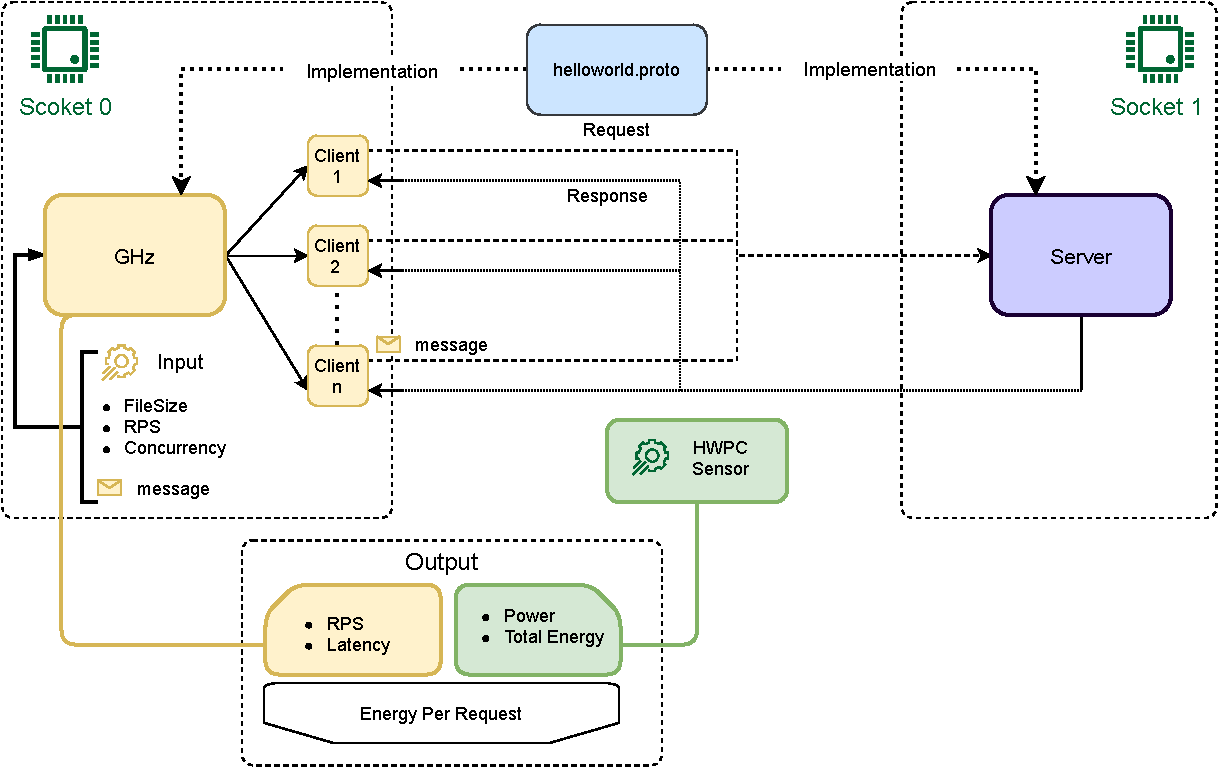
\includegraphics[width=.8\linewidth]{imgs/rpcprotocol}
    \end{center}
    \caption{Experimental software architecture.}\label{fig:rpcprotocol}
\end{figure}



\paragraph{Performances.}
For better accuracy and more details, We use an updated version of the open source RPC benchmarking tool, named GHZ (\url{https://ghz.sh/}).
The modified version allows us to monitor the average power for each request from both the server and the client sides.
The new version is available in the repository.\footnote{\url{https://github.com/chakib-belgaid/energy_ghz}}

\subsubsection{Input Workload}
The purpose of the experiment is to analyze the behavior of different GRPC implementations.
Therefore, we have two kind of worlkoads: \emph{number of clients} is the number of concurrent clients that we want to benchmark (handled by the GHZ client) and the \emph{payload} reflects the size of each request (varies from 50 Bytes up to 10 MB).
The client consumes the protocol description found in the file \texttt{helloworld.proto} to generate an implementation for the message and then forks multiple instances that send the same request to the server.

\subsubsection*{Candidates}
The server implementations are based on the official implementation by Google for most of the languages.
Each server uses 16 cores and is limited to 512\,MB of RAM.
Each implementation is packaged as a Docker image, which will allow us to add new implementations easily.

\subsubsection{Extension}
For the sake of experimental extensibility, we provide a GitHub repository that contains the implementation of all our experiments.\footnote{\url{https://github.com/chakib-belgaid/energy_benchmarking_grpc2}}
Adding a new RPC \textbf{candidate} can be achieved by creating a new Docker image and putting it in a new folder named after the language.
As for the \textbf{workload}, it can be extended easily by adding new files in the folder \textbf{payload}.


\subsection{Results \& Findings}
\paragraph{\textsc{RQ}~1: How do RPC implementations consume with regard to the size of the incoming request?}

The purpose of this question is to study the energy consumption of the RPC server when transferring large objects.
To do so, we send $80,000$ requests to the server whose size scales from 10 bytes up to 10 Megabytes, resulting in $10,000$ requests per size per server.
To eliminate extra factors, we let the server handle the rate at which it can answer each request.
However, we put a 20 seconds timeout deadline for each request.
Therefore, our boundary condition is only the number of requests received by the server.
For this experiment, we investigate 4 observable variables:
\begin{enumerate}
    \item the \textsf{average power consumption} during the scenario indicates the overall behavior of the server when working for long durations,
    \item the \textsf{tail latency} for the 99th percentile, which indicates how efficient is the server,
    \item the \textsf{average number of requests per second}, which indicates the average number of clients that the server can handle,
    \item the \textsf{average energy cost} of a single request: unlike the first indicator, this one shows how green is the implementation considering performance.
\end{enumerate}


\begin{figure}[!hbt]
    \begin{center}
        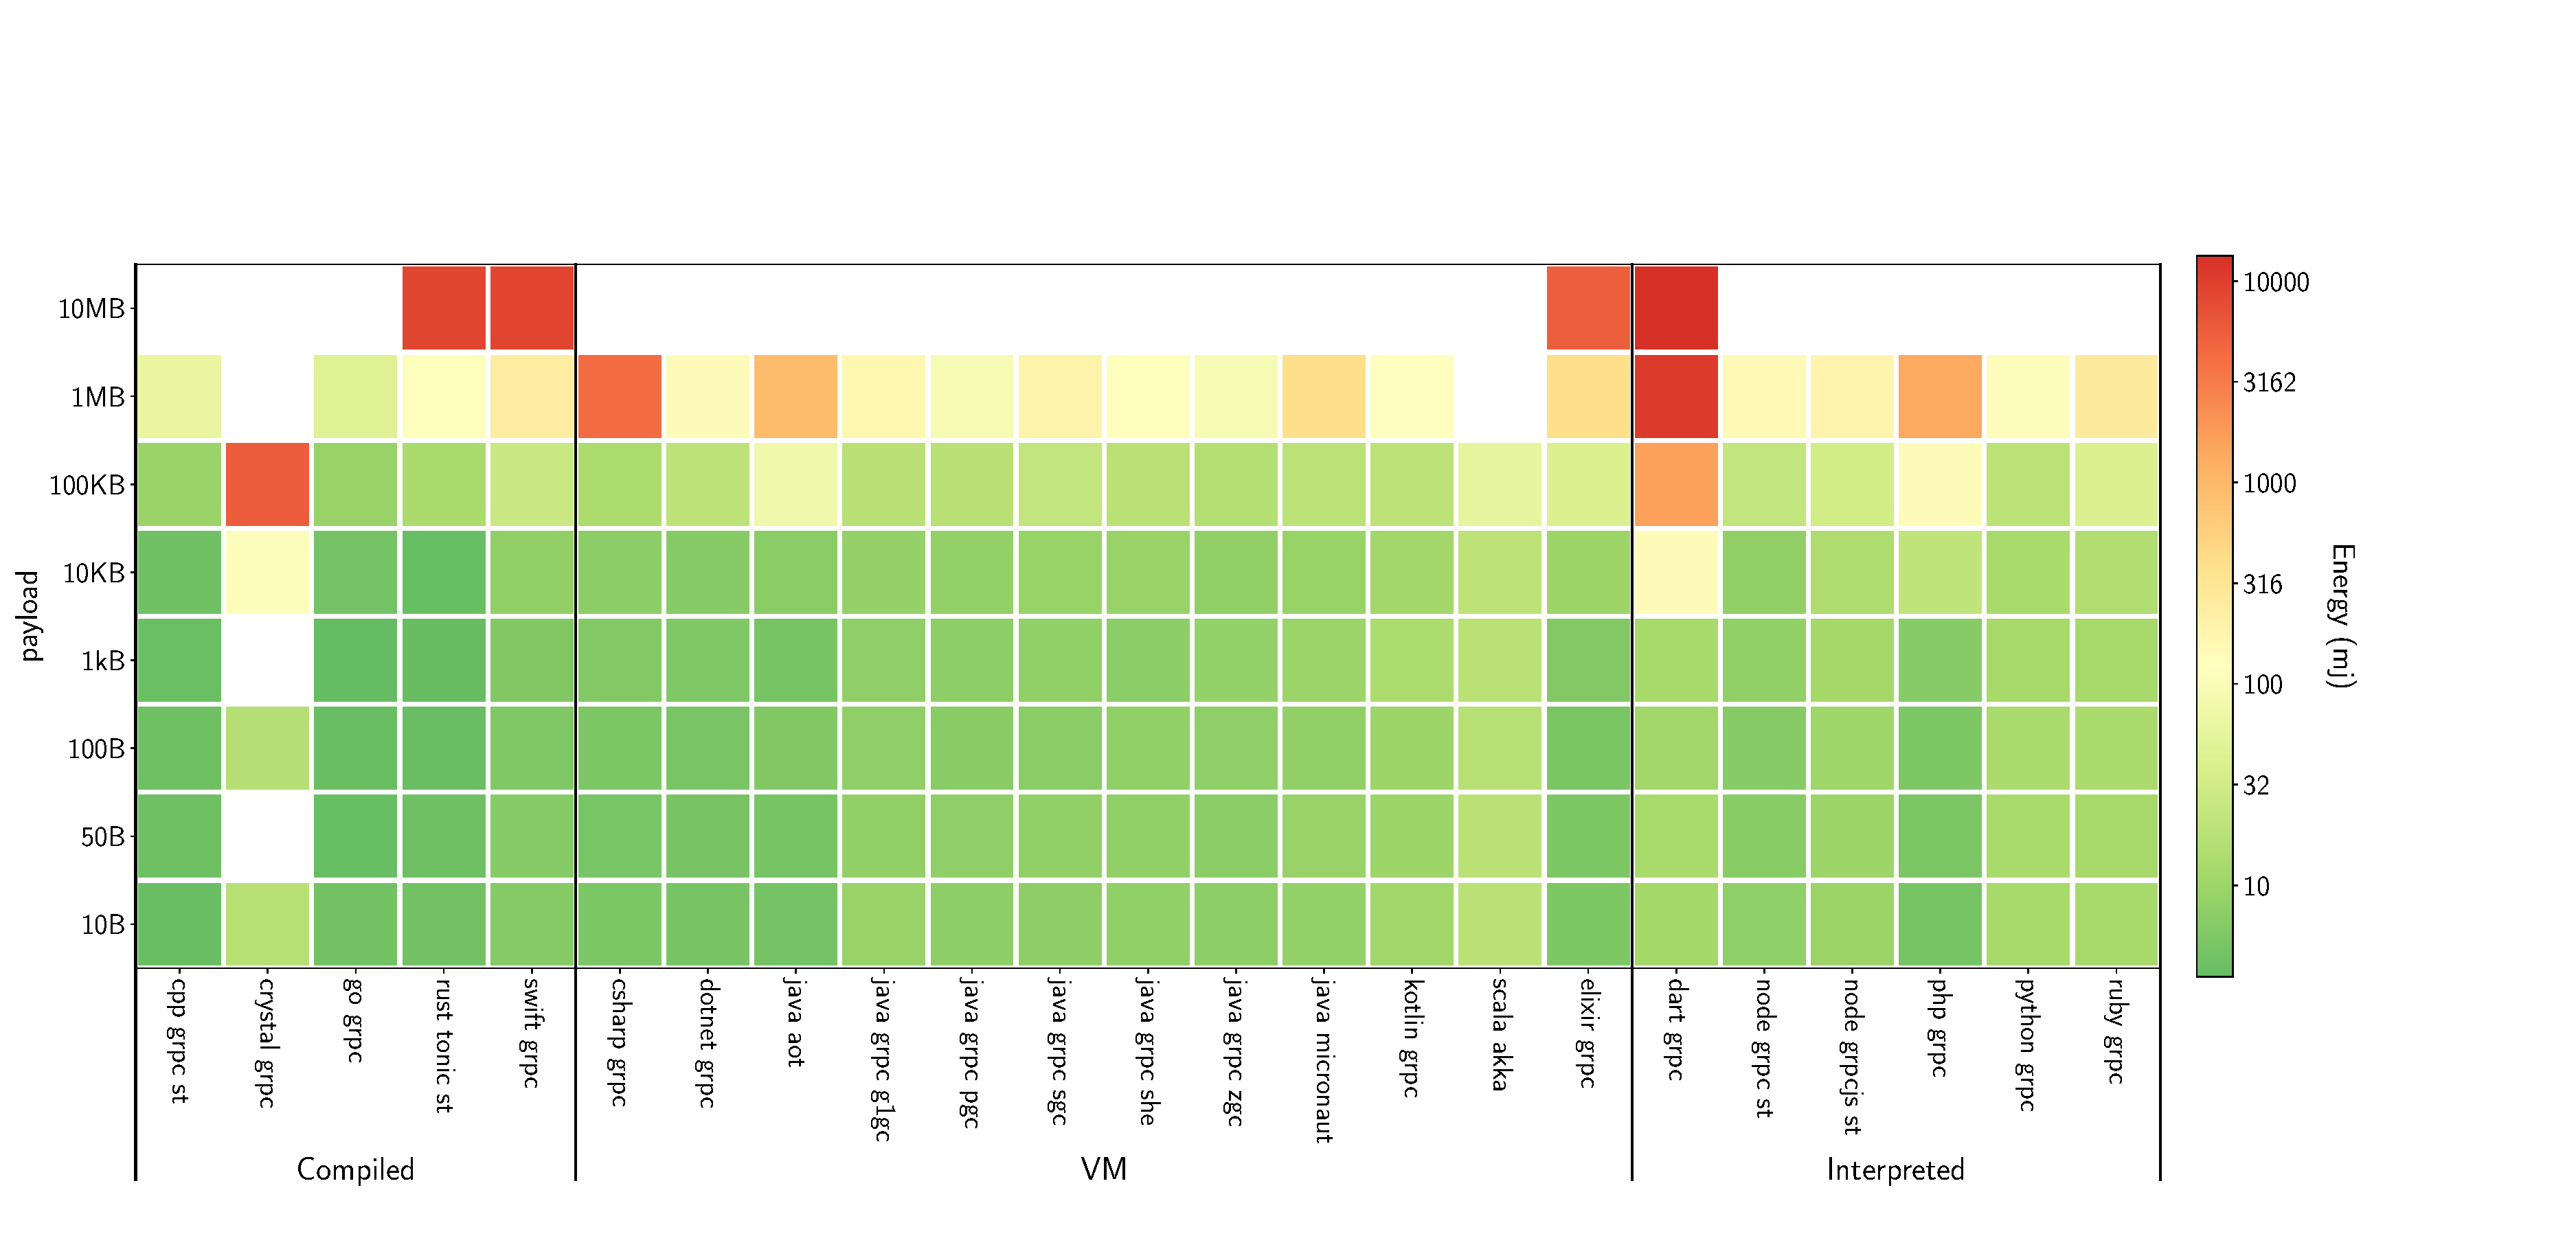
\includegraphics[width=1.2\linewidth]{imgs/energy_cost_payload}
    \end{center}
    \caption{Energy consumption based on the request size}\label{fig:energy_cost_payload}
\end{figure}
Figure~\ref{fig:energy_cost_payload} depicts the overall behavior of each framework based on the size of request (payload).
For each framework, we can distinguish three modes, and they all depend on the payload size:
\begin{enumerate}
    \item \textsf{Stress free} mode when the server has enough resources to satisfy the requests, as they require a memory less than a certain threshold (depends on the language and the platform),
    \item \textsf{Escalation} mode when the requests tend to be bigger, but the server can still manage to handle them, at the price of a change in the energy and performance behaviors,
    \item \textsf{Broken state} mode when the requests are much heavier and the server break—like 10 MB.%ROMAIN unclear to me what this means
\end{enumerate}

\subsubsection{Stress Free Mode}
In this mode, the compiled languages tend to consume fewer resources (average power).
JVM-based languages tend to consume more energy, especially Scala.
However, we do not observe the same behavior when it comes to efficiency.
Unlike the other interpreted programming languages, PHP's performance can be compared to the compiled ones, such as CPP or GO, and even better to some others, such as Swift.
JVM-based languages tend to have better performance than interpreted ones.
Furthermore, OpenJDK has shown more efficiency than GraalVM.
Overall, we can have 3 groups when it comes the cost of each request:
\begin{itemize}
    \item Energy-efficient class: C++, GO, RUST, ELIXIR, and PHP,
    \item Middle class: Most of the interpreted languages and VM-based ones,
    \item Energy-greedy class: Crystal and Scala.
\end{itemize}

\subsubsection{Escalation Mode}
In this mode, the behavior of the server depends on the payload. We observe three cases:
\begin{enumerate}
    \item drop in performances without an increased power source, such as Net core, Java Micronaut, Crystal, and Dart.
    In this case, the server keeps using the same resources, and sometimes less, because it takes more time to handle the fewer requests.
    This class of languages tends to be the most energy-consuming when it comes to the cost per request;
    \item increase in power without affecting the performance, such as Go or.Net.
    The energy consumption of a single request is affected slightly but still increases.
    \item Increase in power and a drop in performance.
    Despite the increase in power consumption, the server becomes slightly slower, which increases the energy cost per request.
    This cost is still better than the first case, which concludes that the servers in the first category are on the verge of breaking.
\end{enumerate}

We can mention the case of Elixir that keeps scaling despite the lack of performance compared to other compiled languages (Go, CPP)..

\subsubsection{Broken state mode }
Only four of the 25 configurations could parse the 10 MB files, and only one of those could achieve a 76\% acceptance rate, which is Elixir. The other 3 had less than a 3\% success rate (Rust, Swift, and Dart).
The rest could be divided into two categories:
\begin{itemize}
    \item \textsf{Timeout} where requests took too much time that the client canceled them, in this category we find most of dynamic codes, such as OpenJDK and Kotlin,
    \item \textsf{Size of request} exceeded the maximum size when the implementation could not handle requests with large size, as observed with .Net, Go, .Net core, CPP, PHP, Scala, Nodejs, Ruby, Python.
\end{itemize}


[\textsc{RQ}~2:] How do RPC implementations react to the number of clients ?
\begin{figure}[!hbt]
    \begin{center}
        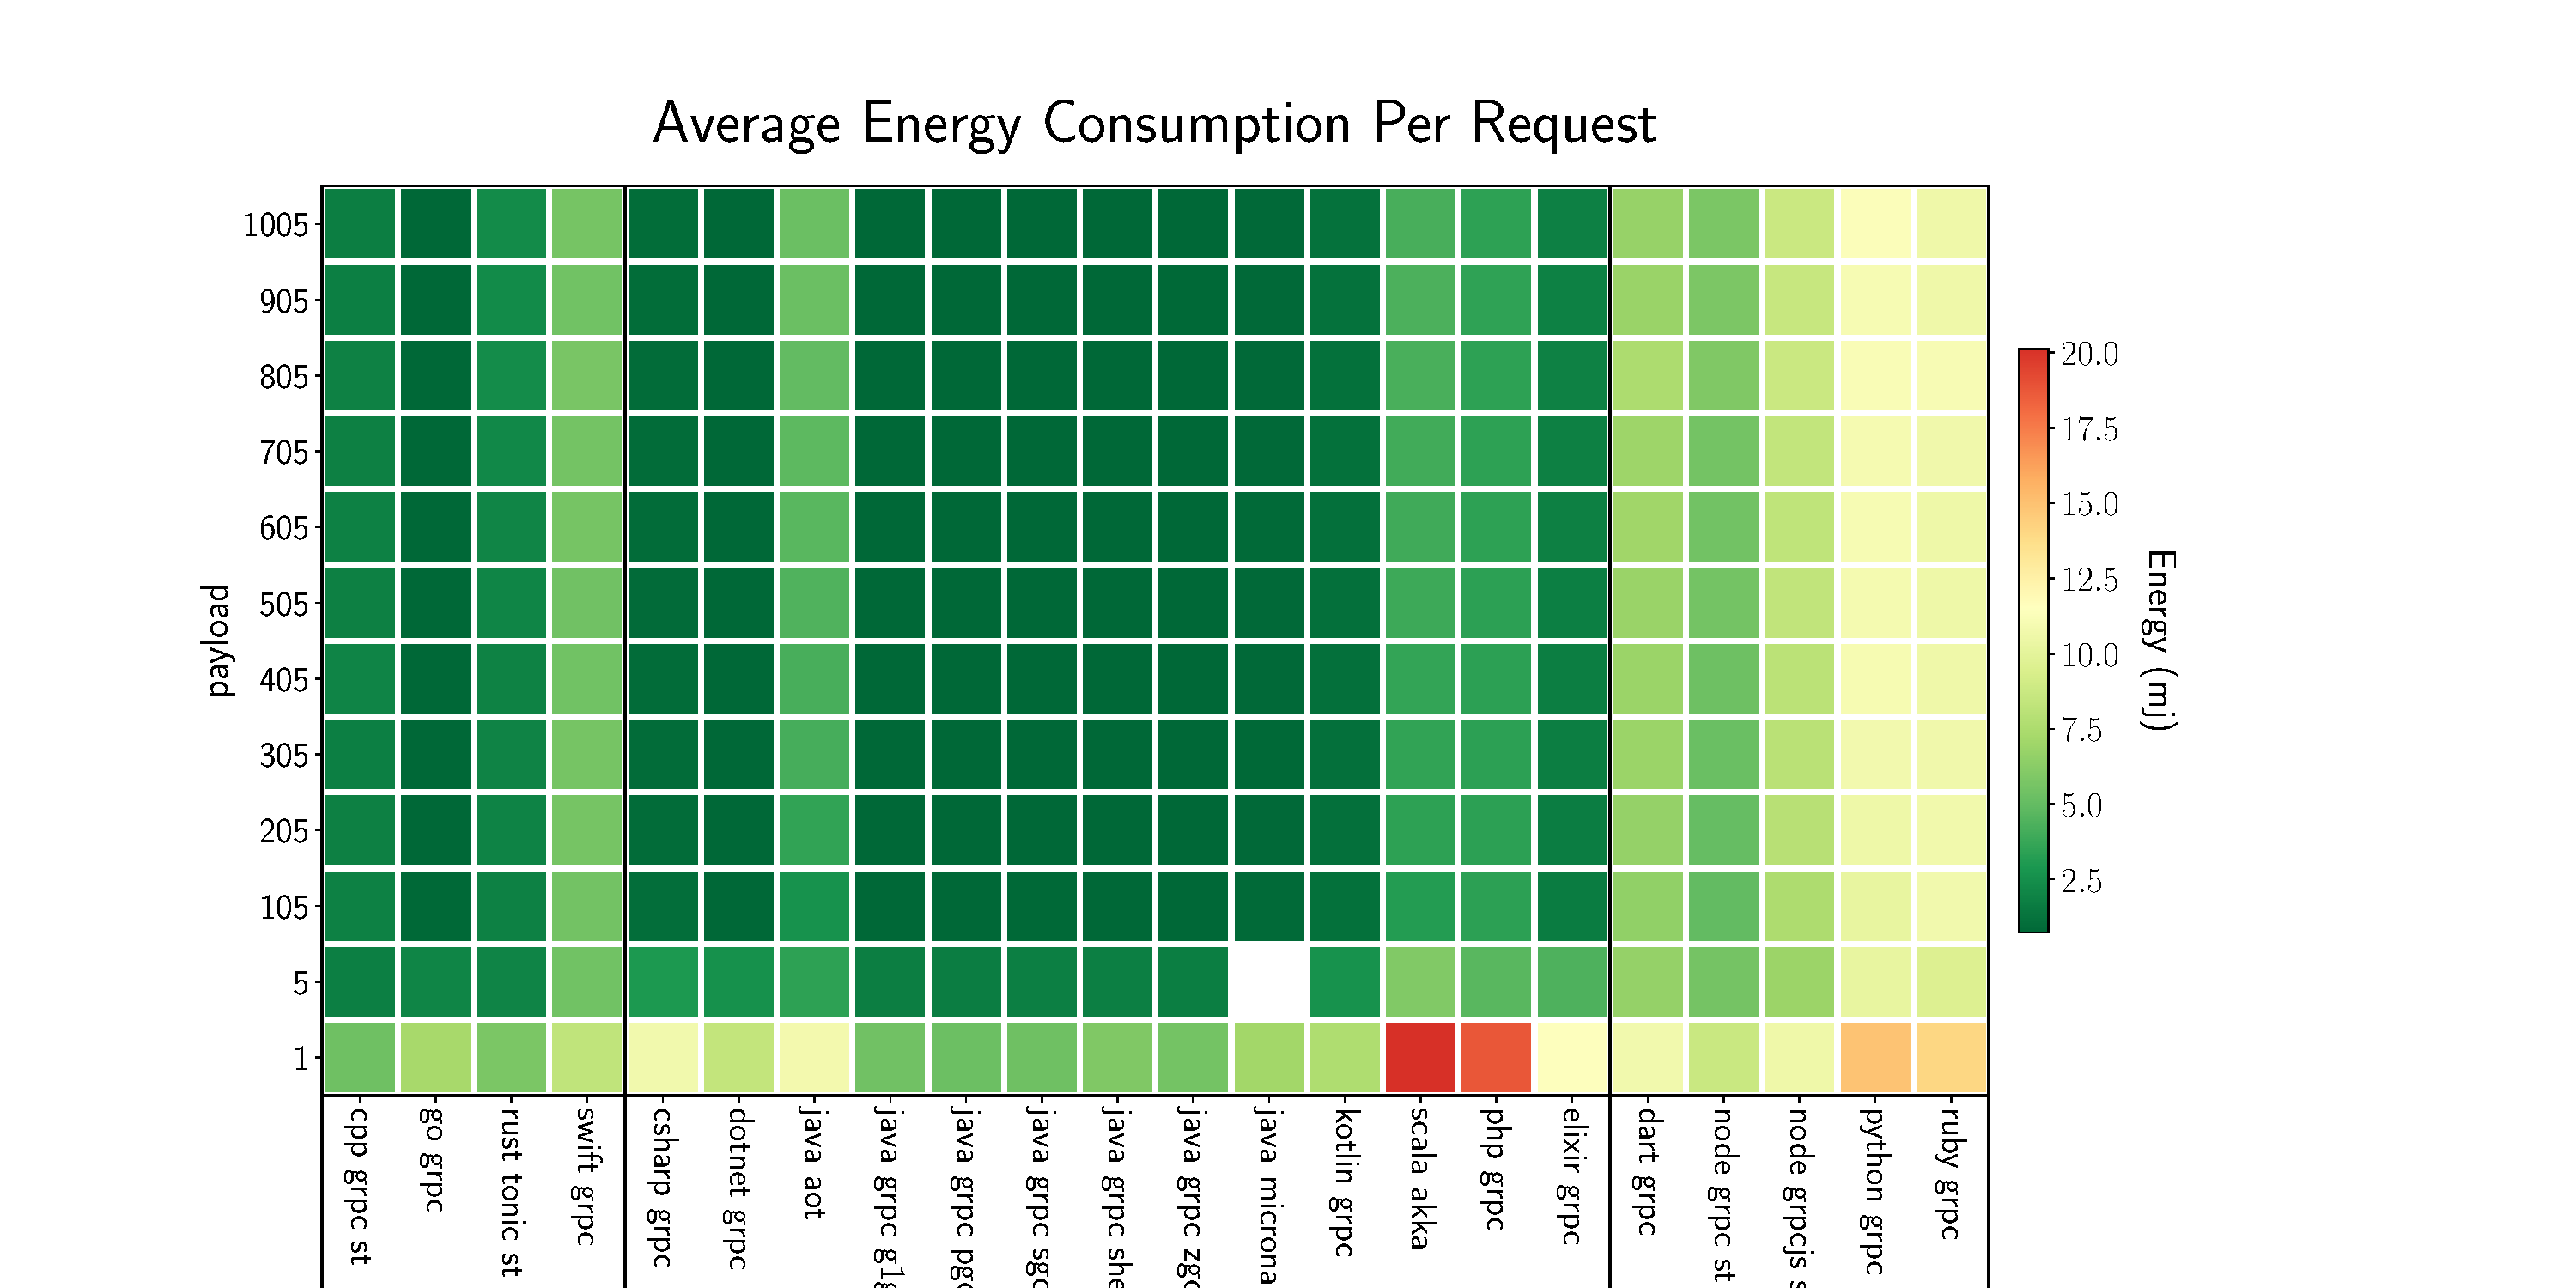
\includegraphics[width=1.2\linewidth]{imgs/energy_cost_clients}
    \end{center}
    \caption{Energy behaviour based on the number of the clients}\label{fig:rpcproenergy_cost_clients}
\end{figure}

\subsubsection{Power behaviour}

\begin{figure}[!hbt]
    \begin{center}
        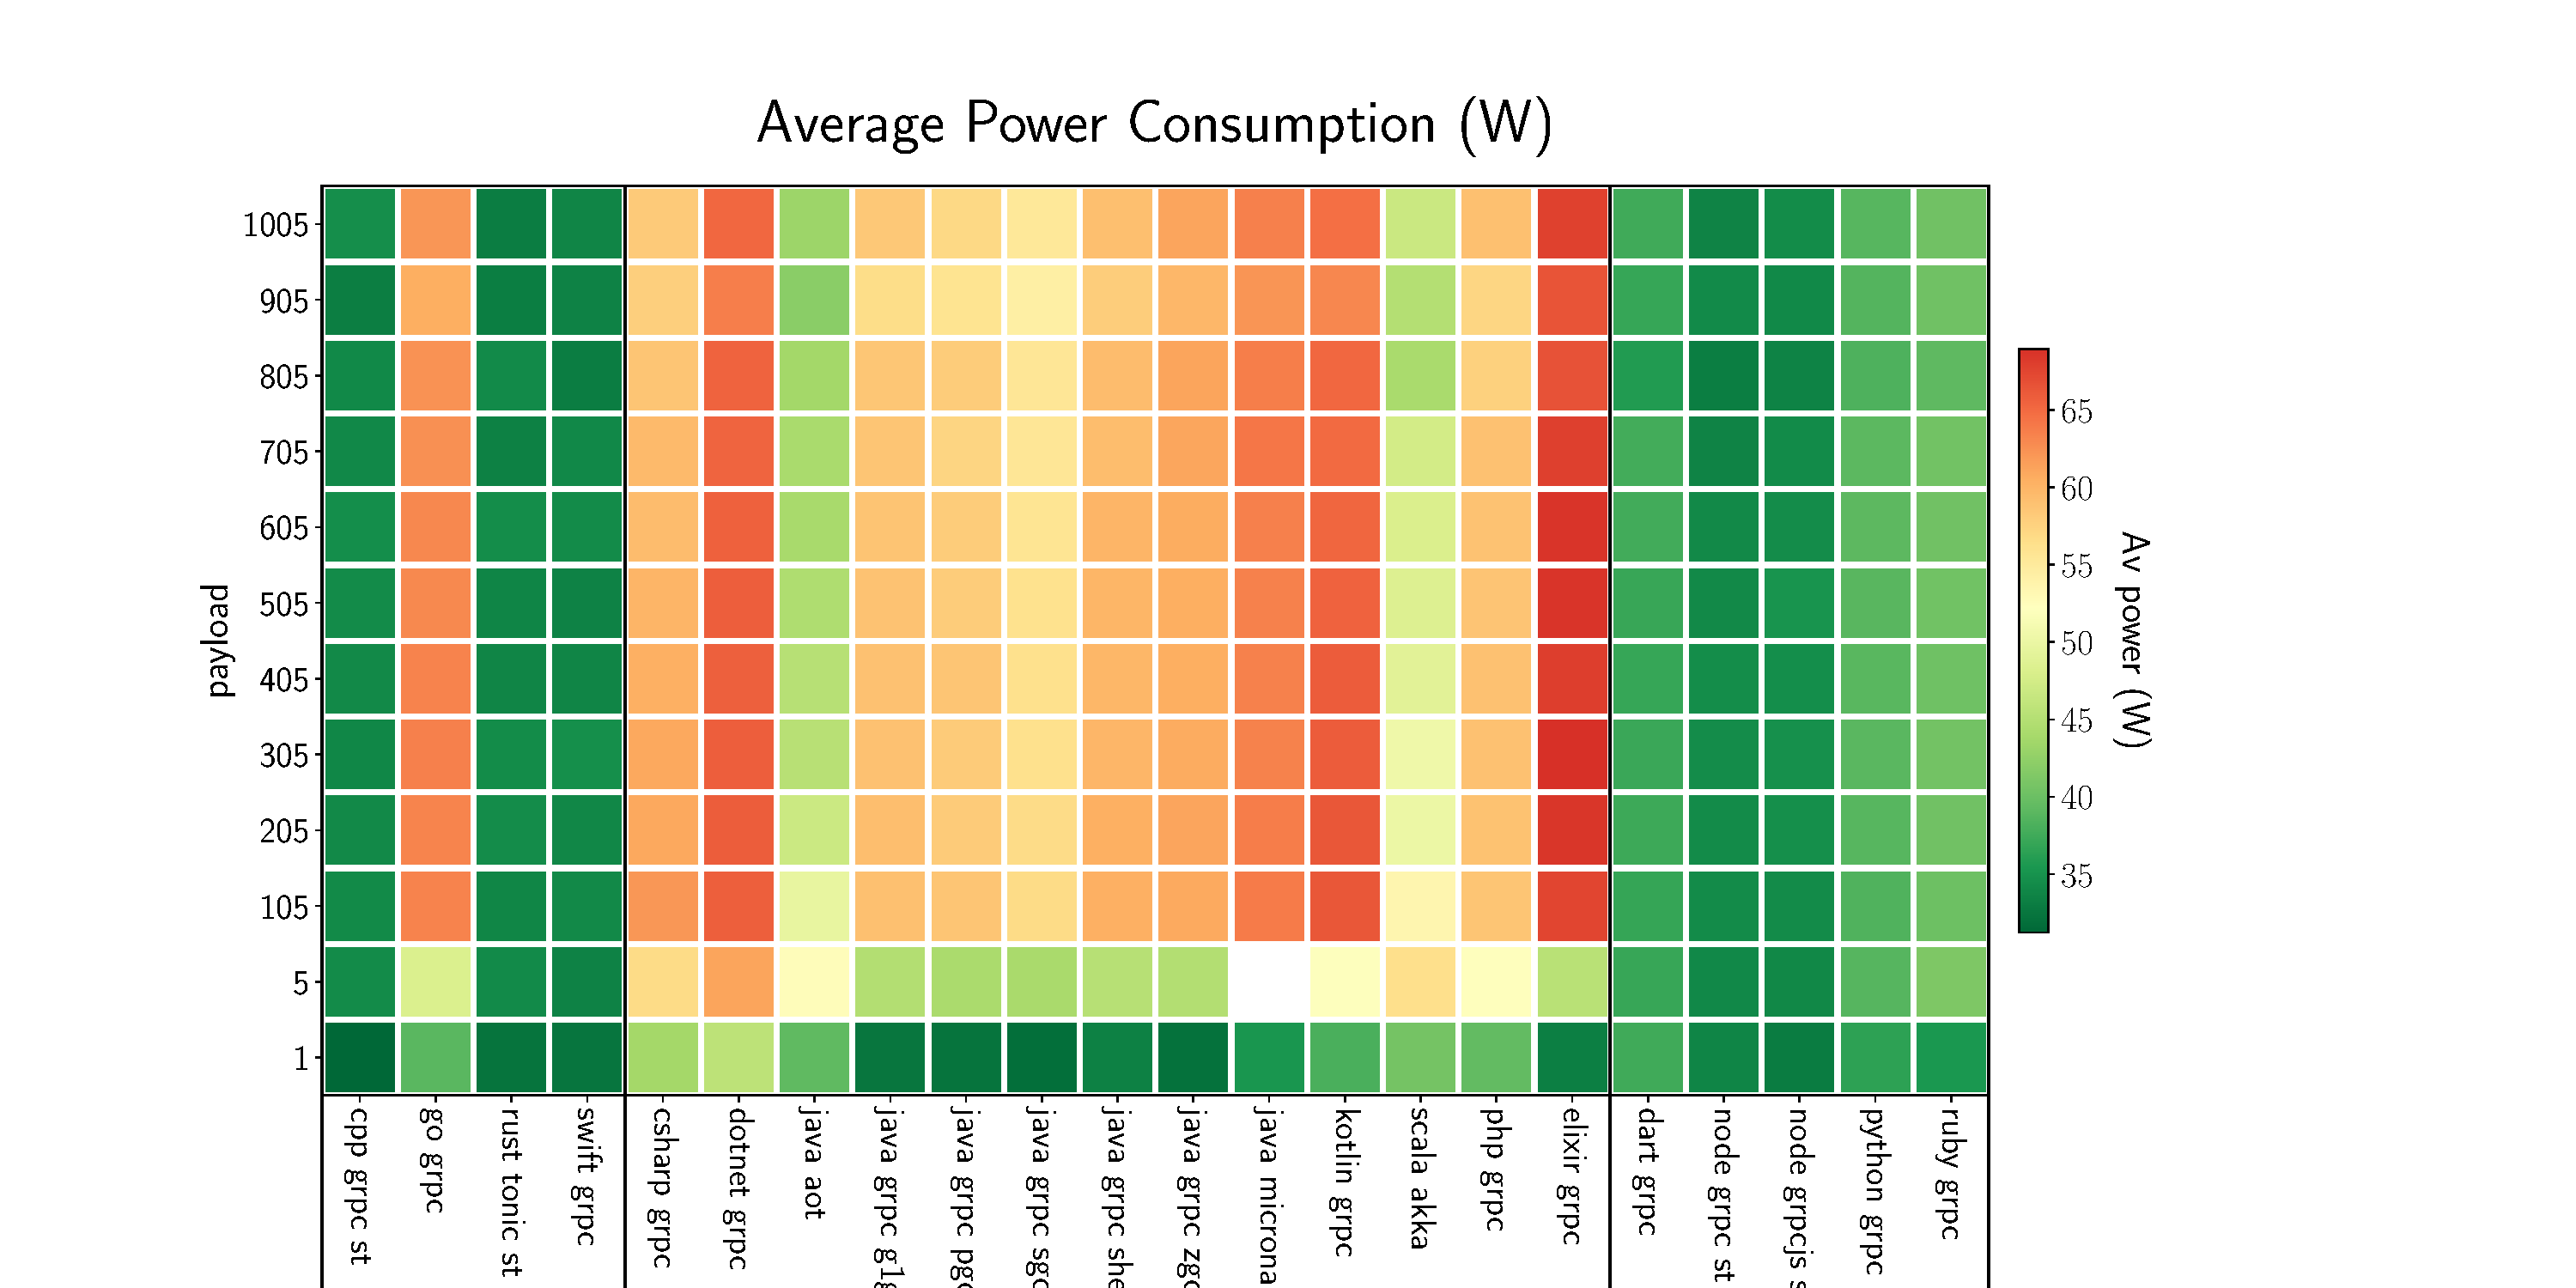
\includegraphics[width=1.2\linewidth]{imgs/power_consumption_clients}
    \end{center}
    \caption{Average power consumption based on the number of the clients}\label{fig:power_consumption_clients}
\end{figure}

\begin{figure}[!hbt]
    \begin{center}
        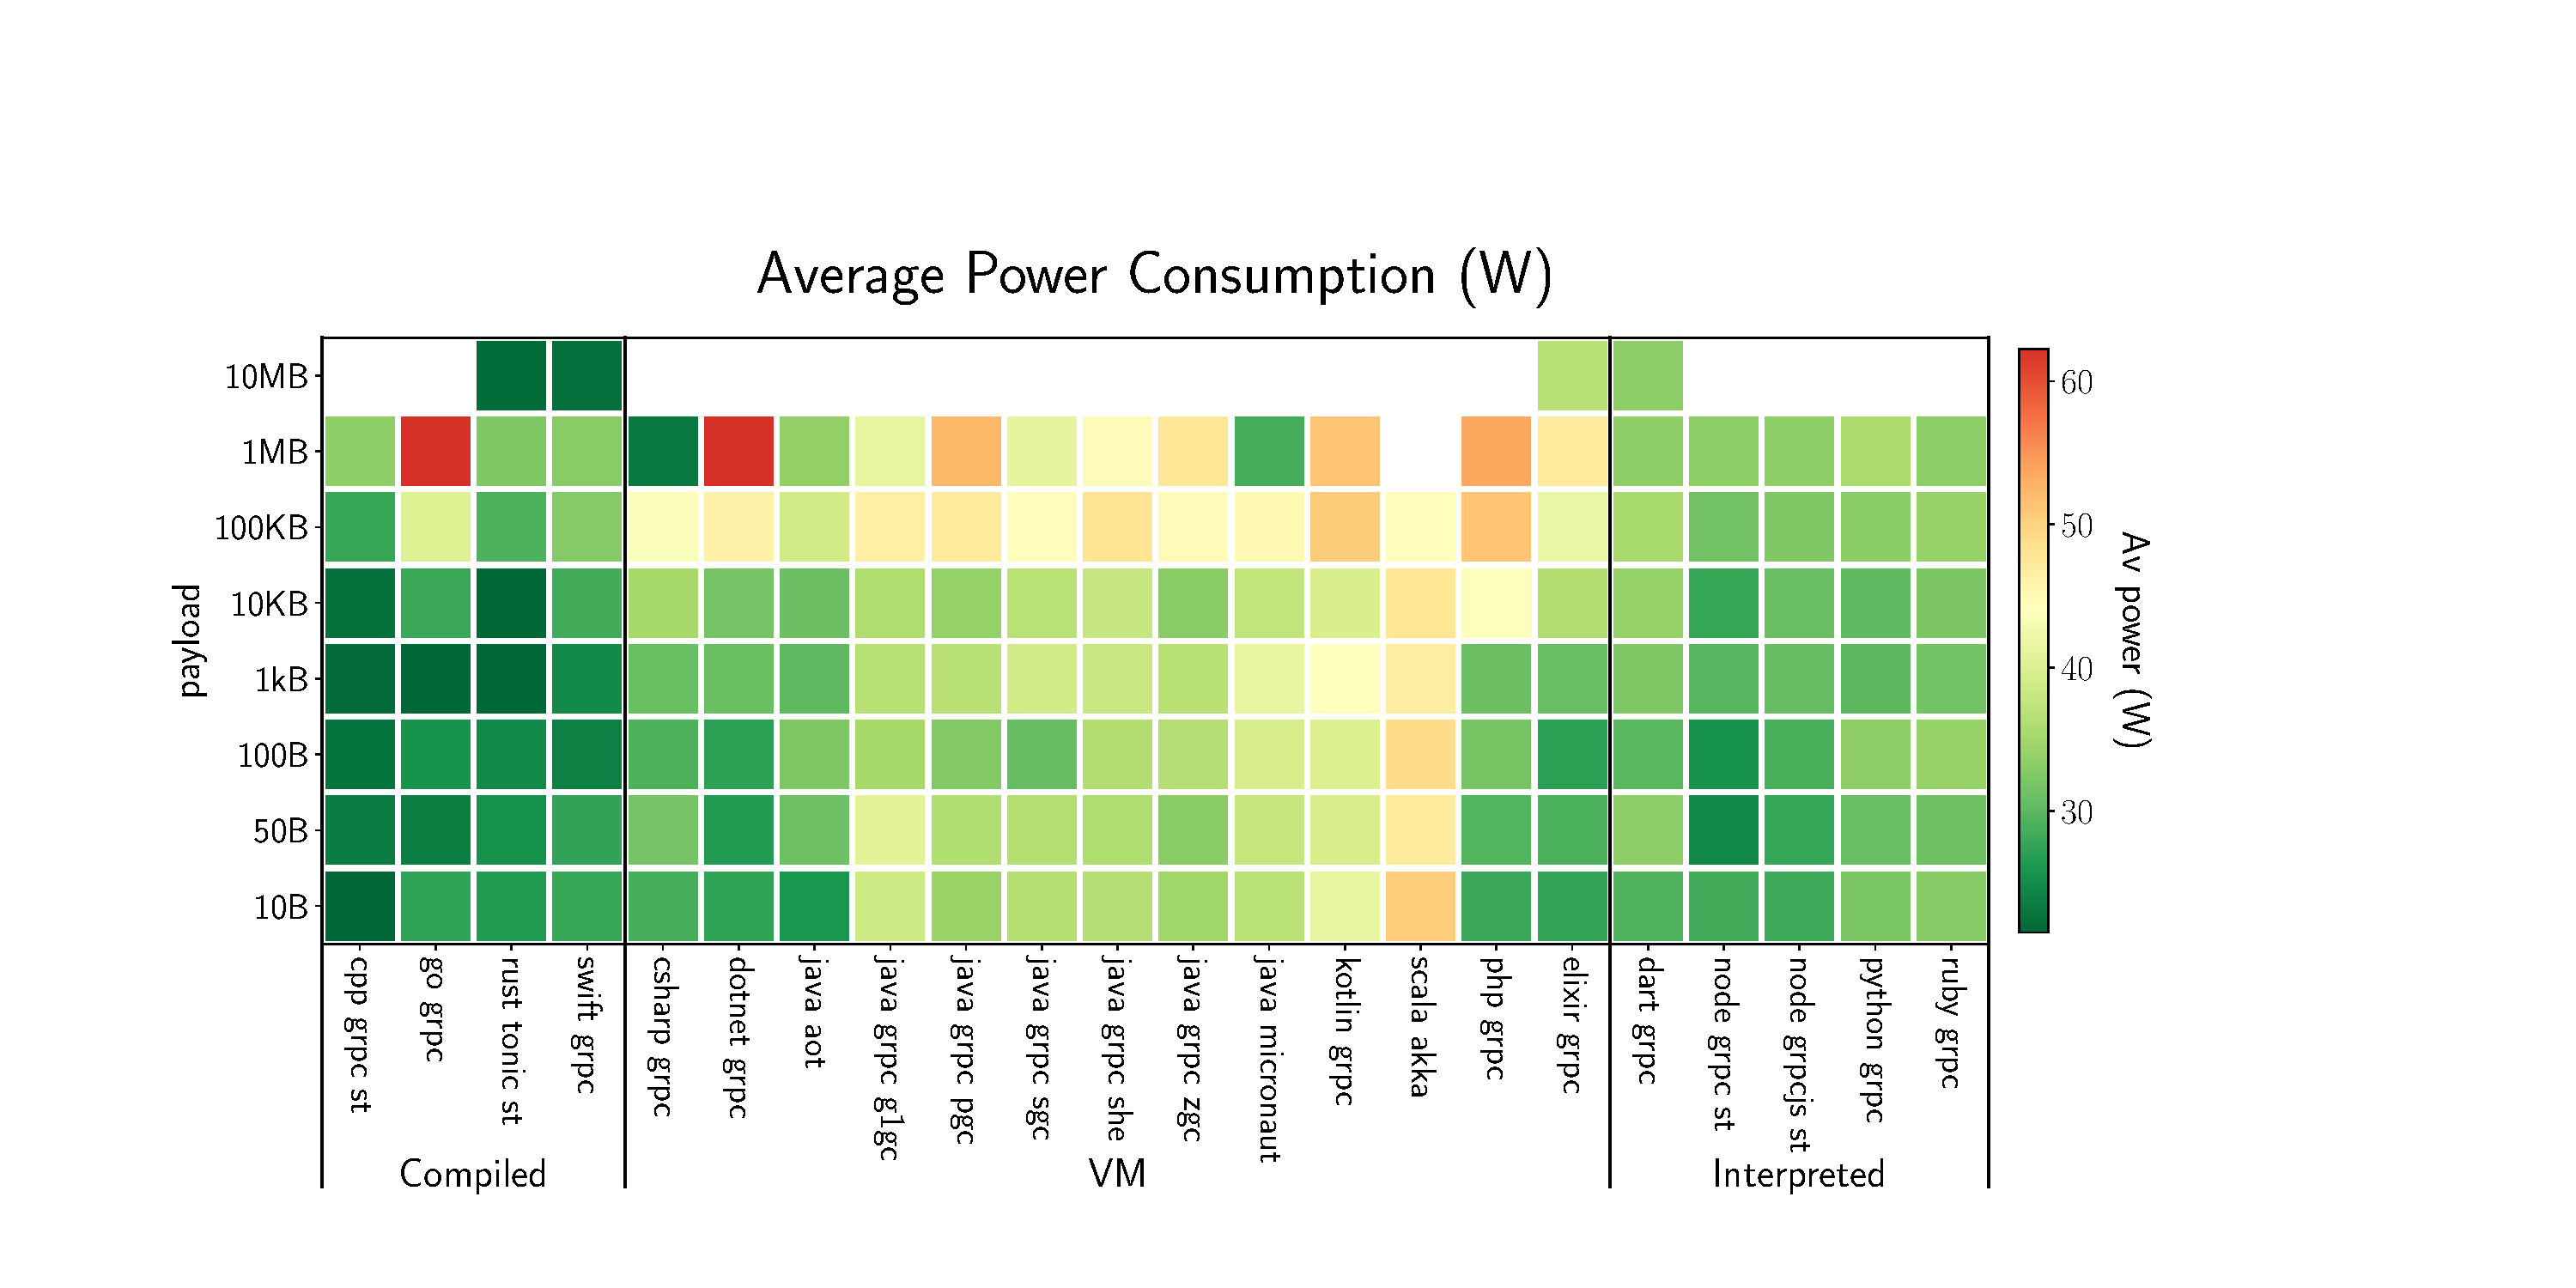
\includegraphics[width=1.2\linewidth]{imgs/power_consumption_payload}
    \end{center}
    \caption{Average power consumption based on the request size}\label{fig:power_consumption_payload}
\end{figure}

Based on the heatmap, we can distinguish two modes:
\begin{itemize}
    \item \textsf{Low number of clients} when the number of concurrent clients is below 100,
    \item \textsf{Moderate to high number of clients} when the number of clients exceeds 100.
\end{itemize}


\paragraph{Lite mode}
The benchmarked implementations can be grouped into two classes:
\begin{enumerate}
    \item \textsf{Energy-efficient frameworks} where most of the framework's power consumption is around 33 Watts.
    \item \textsf{Energy-greedy frameworks} where the average power consumption is higher than 37 Watts.
\end{enumerate}

In each programming category, we observe both energy-efficient and energy-greedy behaviors.
Therefore, we conclude that it depends more on the implementation of the library itself than on the category of the programming language.
Scala and Kotlin are excellent examples to support this hypothesis, as both of them run on the same virtual machine as Java (OpenJDK 16.1).
Yet, their average power is 130\% higher than the Java implementation.

\paragraph{Stressed mode}
Although the same classes remained the same, not all the languages had the same evolution, and here we can clearly observe a correlation with the category of the programming language rather than the implementation itself.
We can easily point out that the average amount of power used by VM-based languages doubles when they have more than 100 clients at the same time.
Except PHP, all the interpreted and compiled languages preserved their energetic behaviour.
Our hypothesis points to the JIT, since it compiles the code and makes it run faster, hence stressing the CPU.
An interesting behavior has been noticed for the GraalVM: the decrease in energy consumption when increasing the number of clients.
This is related to the performance drop, which was probably due to the bottleneck situation where the GraalVM could not handle more than 100 clients simultaneously.

\subsubsection{Performance Behaviour}
In this section, we study only the number of requests per second processed by the server without looking at its energy.
We consider three observable variables:
\begin{itemize}
    \item \textsf{Satisfaction ratio}: how many requests have been satisfied among the total requests,
    \item \textsf{Request Per Seconds}: The number of the requests that have been answered from the server,
    \item \textsf{Tail Latency at 99\%}: one of the best metrics to evaluate the performances of a server.
\end{itemize}

\paragraph{Satisfaction ratio}
Most of the considered frameworks satisfy all the requests by either reducing the number of requests per second or increasing the processing time.
However, there are some frameworks that have chosen a different approach, such as Dart or Scala, where the choice was to keep a certain limit of latency even if not all the requests are answered.
Furthermore, we tend to observe this behavior among other frameworks, such as Python or Asynchronous NodeJS, when the number of clients exceeds 800.

\paragraph{RPS}
\begin{figure}[!hbt]
    \begin{center}
        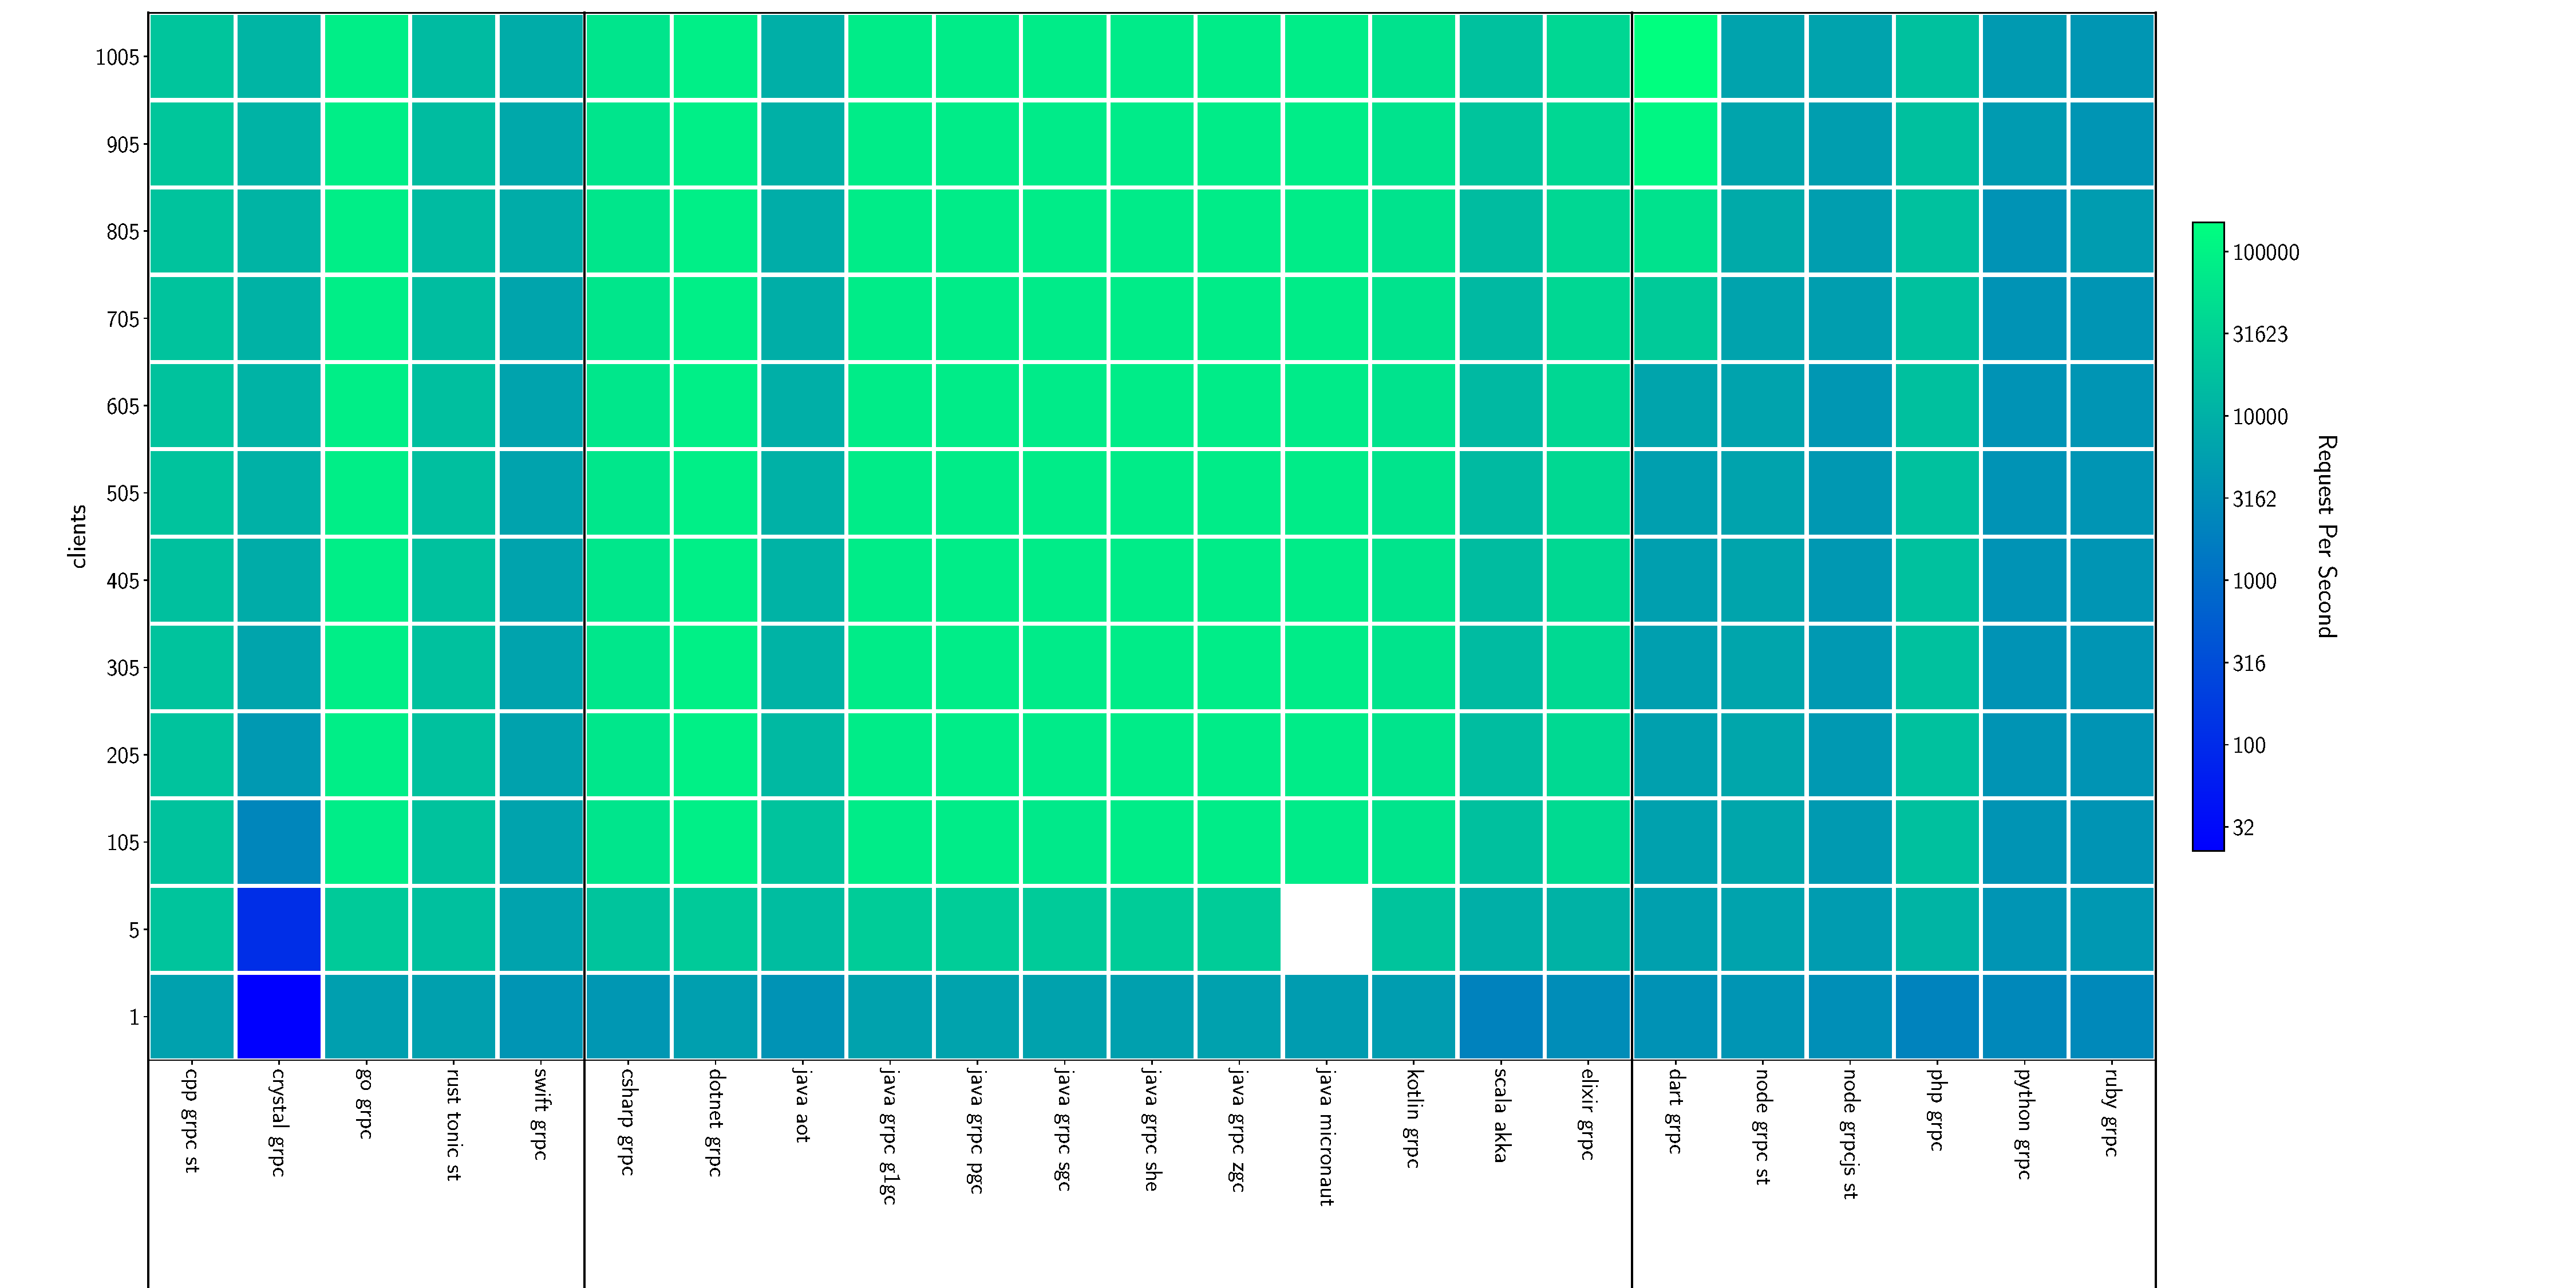
\includegraphics[width=1.2\linewidth]{imgs/rps_clients}
    \end{center}
    \caption{Number of requests per second based on the number of clients}\label{fig:rps_clients}
\end{figure}

\begin{figure}[!hbt]
    \begin{center}
        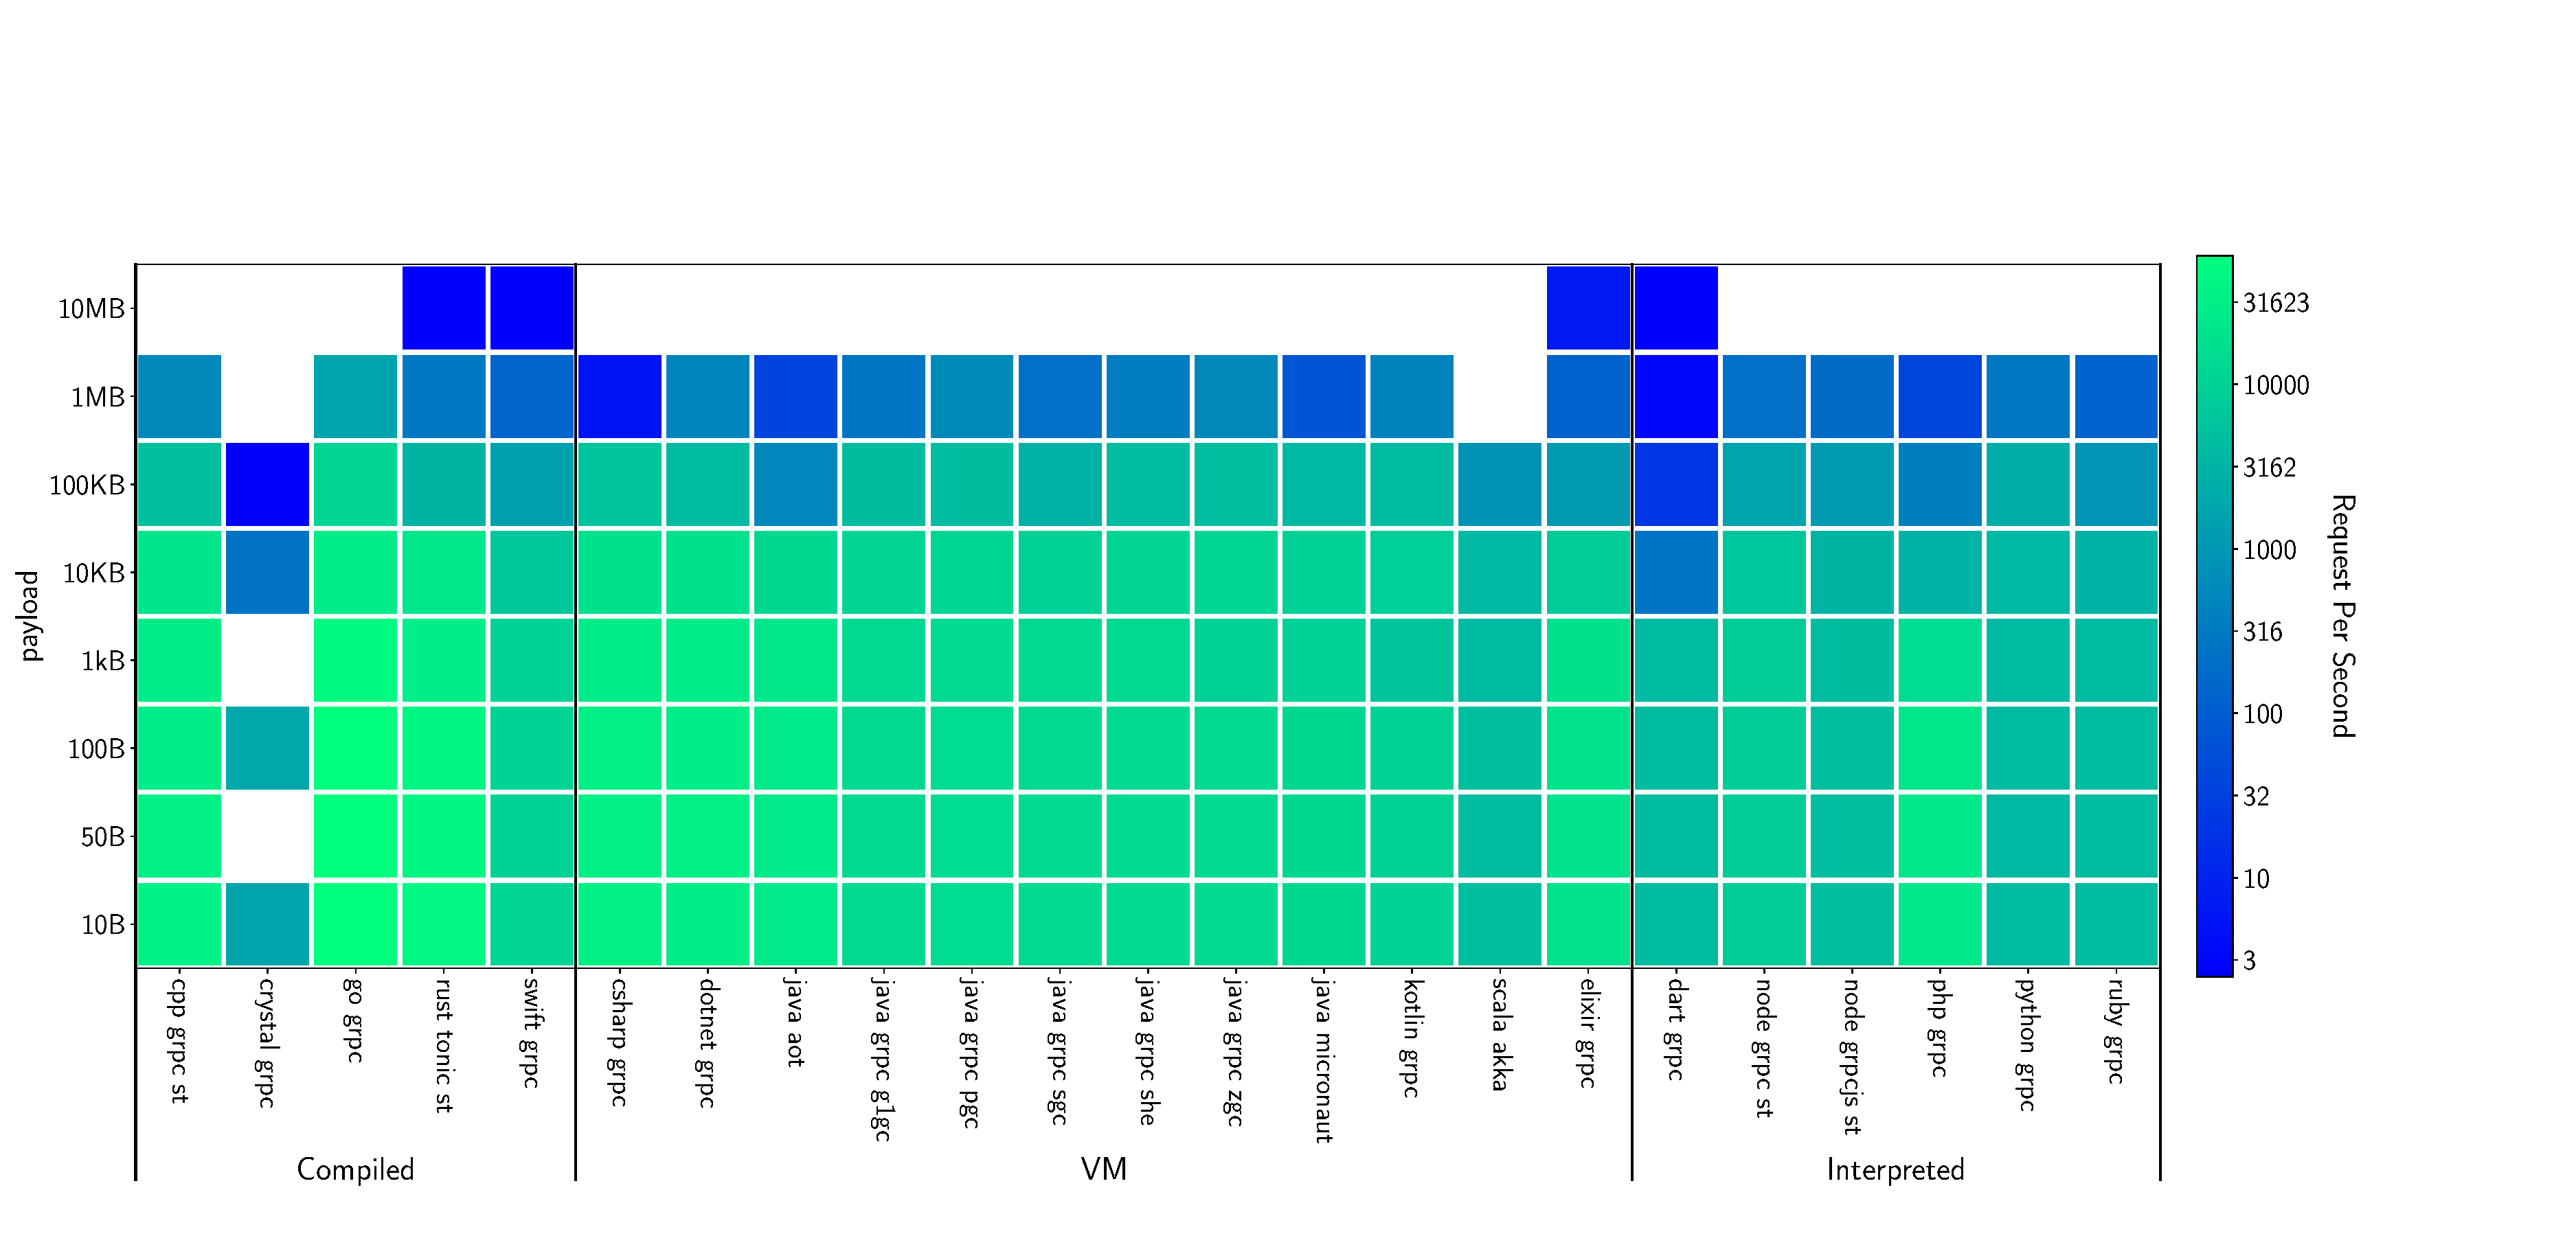
\includegraphics[width=1.2\linewidth]{imgs/rps_payload}
    \end{center}
    \caption{Number of requests per second based on the request size}\label{fig:rps_payload}
\end{figure}
Most of the servers hit their RPS limit after 5 clients and 100 clients for VM-based servers, and after this the number keeps constant, which will decrease the average RPS per client.
. The Net server is the most performant, followed by Java and Go, while Python and Ruby are the least performant.

\paragraph{Tail Latency}
Even if the number of requests per second goes up, that doesn't mean the latency will go down.
As one can notice in figure~\ref{fig:tail99_clients}, until the 1000 clients, Go provides the least latency besides.Net.
GraalVM provides the highest average latency.
However, Dart tends to become slower when we increase the number of clients, until we pass the 600 simultaneous clients, and then it changes its behavior. Instead of satisfying most of the requests, it notifies the clients directly that the server is saturated, resulting in a drop in satisfaction ratio and an amelioration in average latency.

\begin{figure}[!hbt]
    \begin{center}
        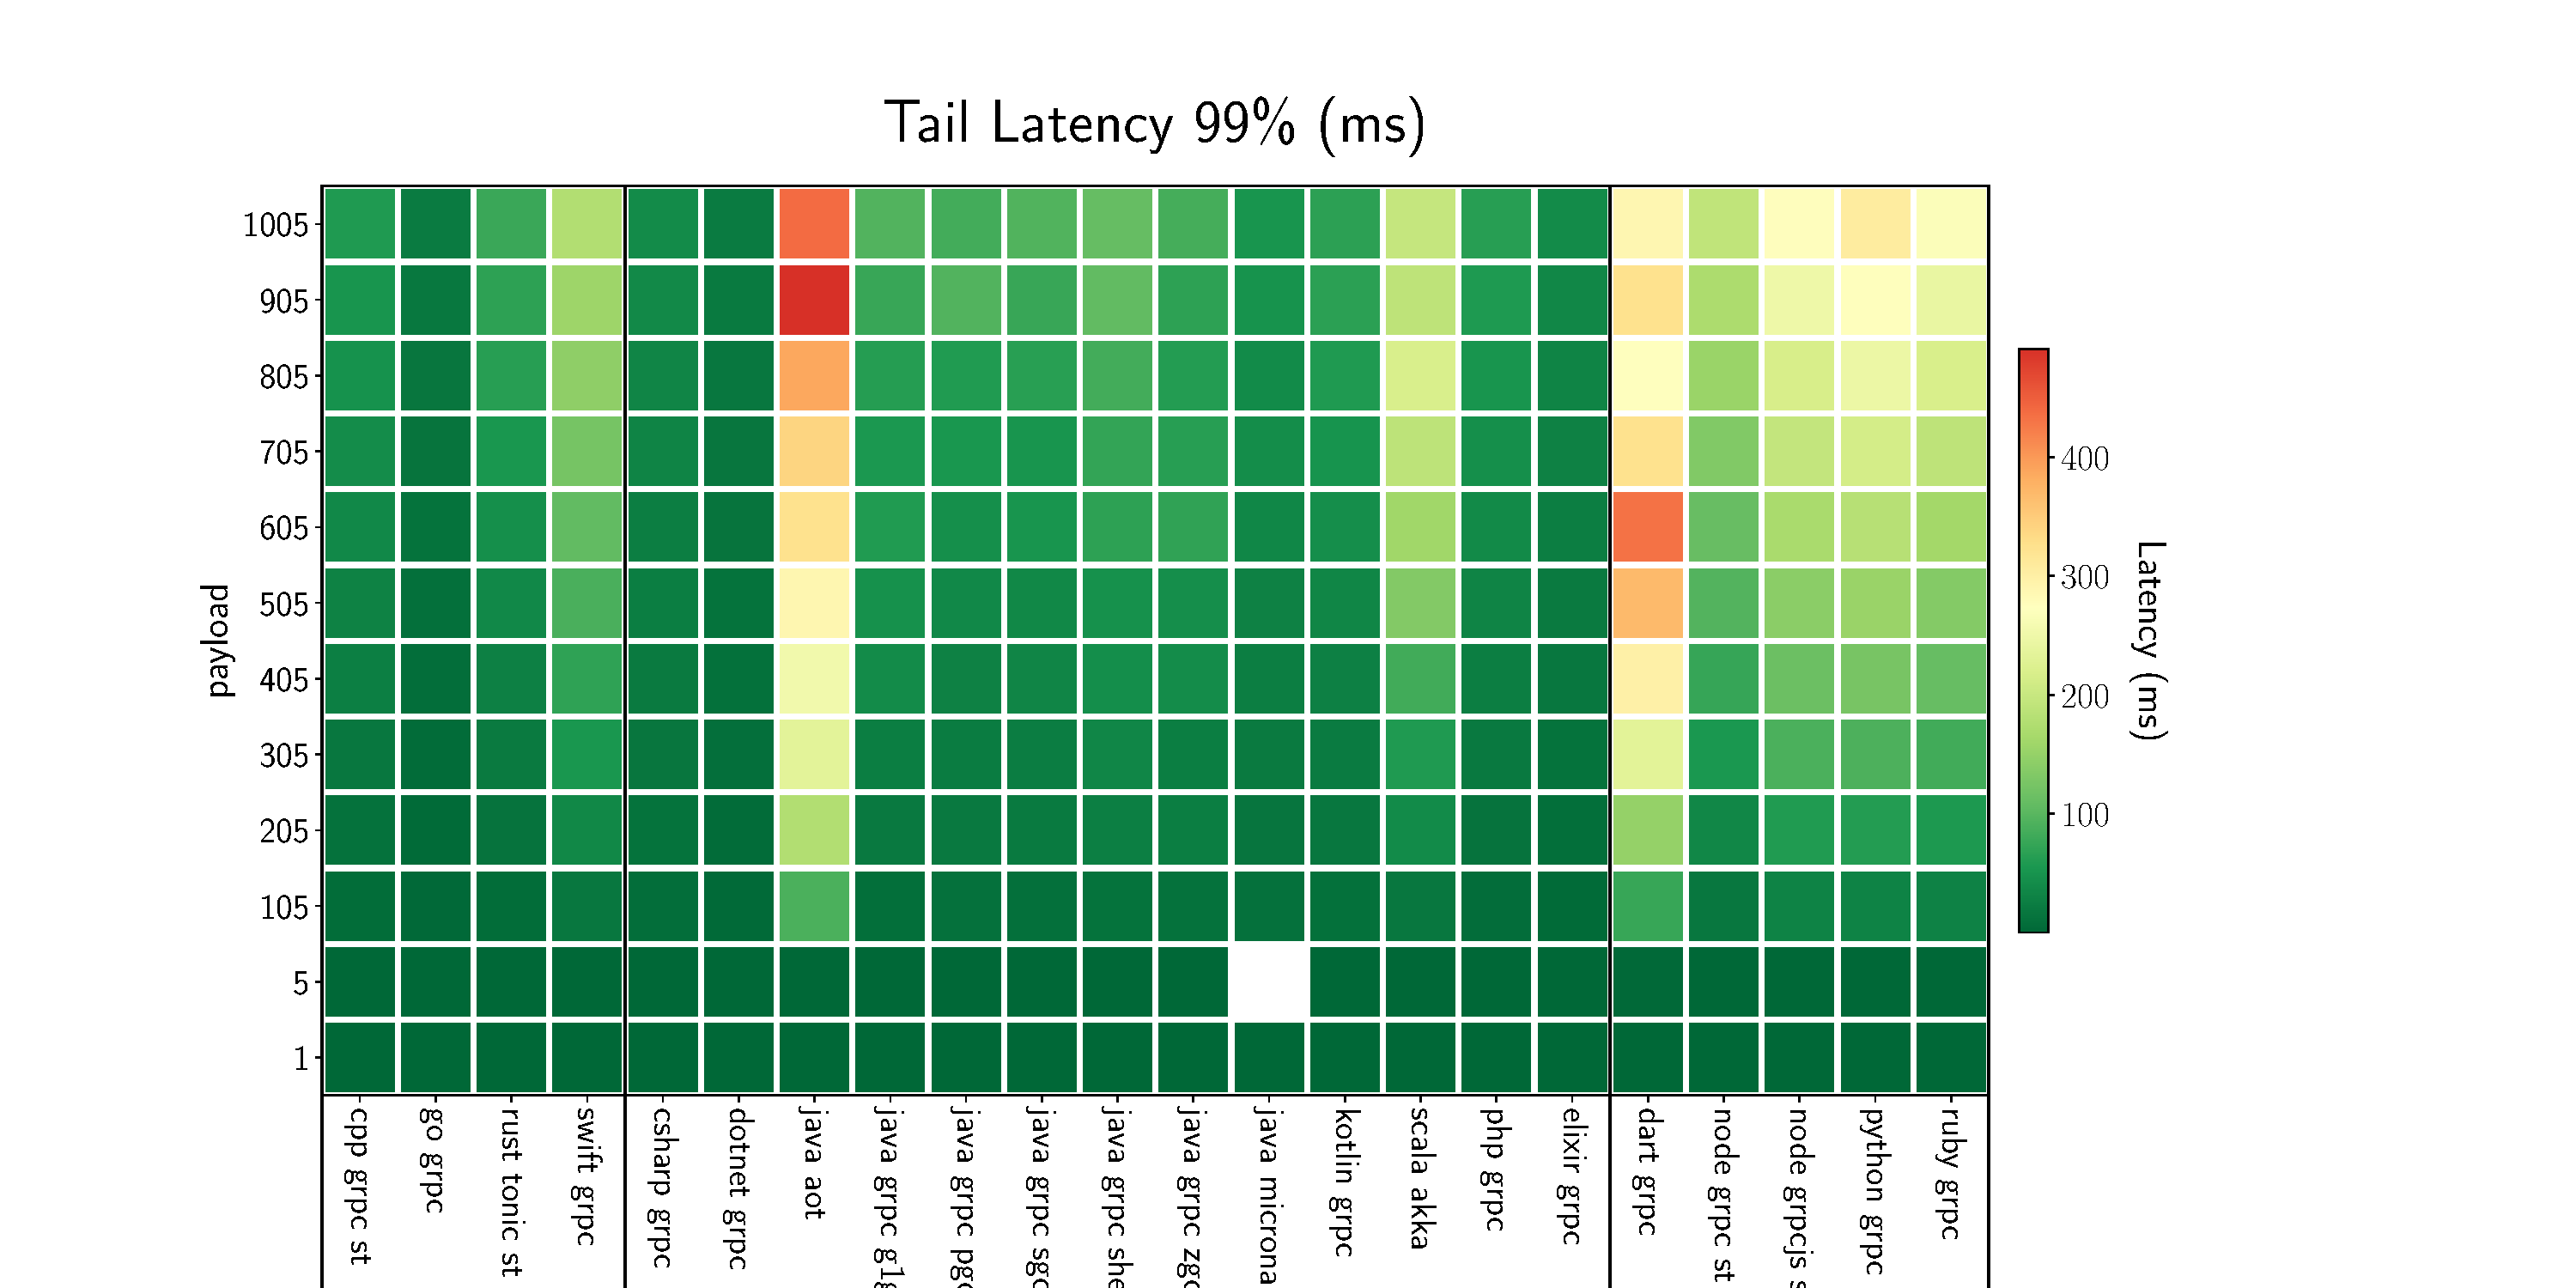
\includegraphics[width=1.2\linewidth]{imgs/tail99_clients}
    \end{center}
    \caption{Tail latency (99\%) based on the number of clients}\label{fig:tail99_clients}
\end{figure}


\begin{figure}[!hbt]
    \begin{center}
        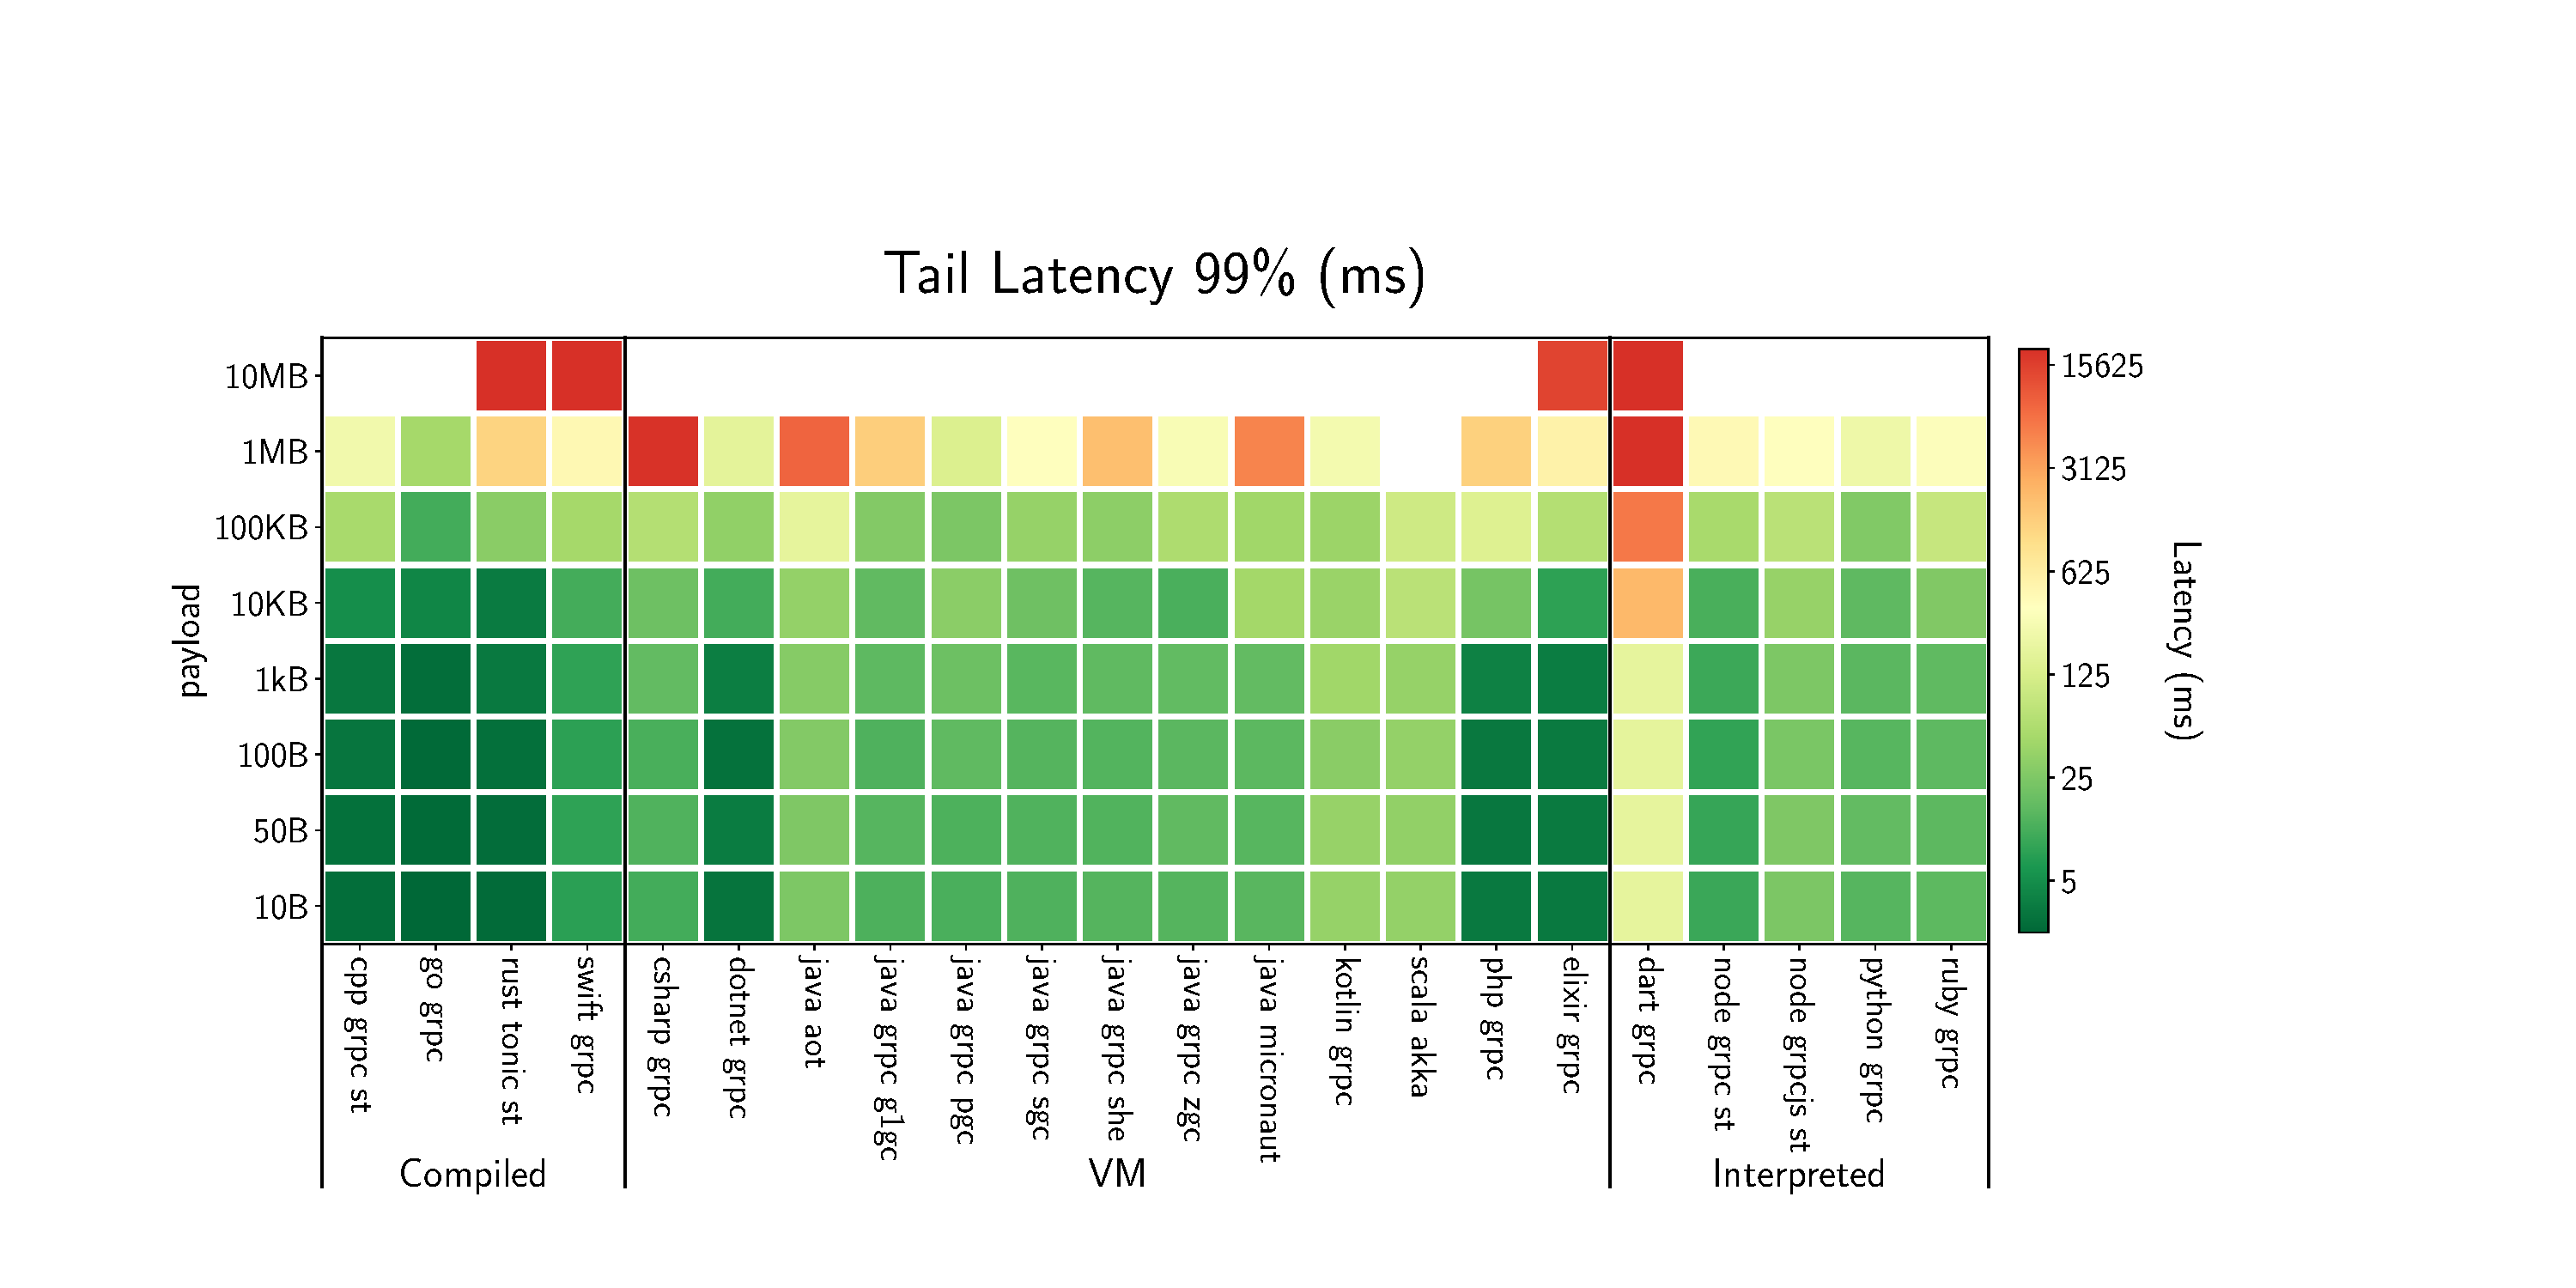
\includegraphics[width=1.2\linewidth]{imgs/tail99_payload}
    \end{center}
    \caption{Tail latency (99\%) based on the request size}\label{fig:tail99_payload}
\end{figure}


\subsubsection{Energy Per Request}
Now, after we made a separation between the energy and the performances, we have seen that most of the performance servers tend to be energy-greedy, so we propose to investigate this trade-off between energy and performances.
To do so, we report the average cost of a single request in joules.
Except GraalVM when the cost of the a single request increases with when we add more clients, all the frameworks report on a constant cost, Java, .net and go are the most energy efficient, while Python and Ruby may cost up to 10x more.
Therefore, we conclude that the number of clients does not significantly impact the energy consumption.
Then, we study how the payload size of the requests impacts the energy consumption of the framework.

% \subsection{Threads to Validity \note{missing}}



\subsection{Conclusion \note{missing}}
